\documentclass[11pt]{article}
\usepackage{geometry,marginnote} % Pour passer au format A4
\geometry{hmargin=1cm, vmargin=1cm} % 

% Page et encodage
\usepackage[T1]{fontenc} % Use 8-bit encoding that has 256 glyphs
\usepackage[english,french]{babel} % Français et anglais
\usepackage[utf8]{inputenc} 

\usepackage{lmodern,numprint}
\setlength\parindent{0pt}

% Graphiques
\usepackage{graphicx,float,grffile,units}
\usepackage{tikz,pst-eucl,pst-plot,pstricks,pst-node,pstricks-add,pst-fun} 

% Maths et divers
\usepackage{amsmath,amsfonts,amssymb,amsthm,verbatim}
\usepackage{multicol,enumitem,url,eurosym,gensymb,tabularx}

\DeclareUnicodeCharacter{20AC}{\euro}



% Sections
\usepackage{sectsty} % Allows customizing section commands
\allsectionsfont{\centering \normalfont\scshape}

% Tête et pied de page
\usepackage{fancyhdr} \pagestyle{fancyplain} \fancyhead{} \fancyfoot{}

\renewcommand{\headrulewidth}{0pt} % Remove header underlines
\renewcommand{\footrulewidth}{0pt} % Remove footer underlines

\newcommand{\horrule}[1]{\rule{\linewidth}{#1}} % Create horizontal rule command with 1 argument of height

\newcommand{\Pointilles}[1][3]{%
  \multido{}{#1}{\makebox[\linewidth]{\dotfill}\\[\parskip]
}}

\newtheorem{Definition}{Définition}

\usepackage{siunitx}
\sisetup{
    detect-all,
    output-decimal-marker={,},
    group-minimum-digits = 3,
    group-separator={~},
    number-unit-separator={~},
    inter-unit-product={~}
}

\setlength{\columnseprule}{1pt}

\usepackage{tabularx}

\begin{document}

\begin{titlepage}

  \center % Center everything on the page

  \textsc{\LARGE Collège Faubert}\\[2cm] % Name of your university/college
  %\textsc{\Large }\\[0.5cm] % Major heading such as course name
  \textsc{\large Villefranche}\\[2cm] % Minor heading such as course title
 
 \horrule{2px}

 \vspace{1cm}

 { \Huge \bfseries Brevet blanc}\\[2cm] % Title of your document
 { \Huge \bfseries Mathématiques}\\[2cm] % Title of your document
 {\large \bfseries 2022}\\[2cm] 

 \horrule{2px}

\begin{itemize}
    \item \textsc{Exercice 1} - 16 points     
    \item \textsc{Exercice 2} - 21 points 
    \item \textsc{Exercice 3} -  8 points 
    \item \textsc{Exercice 4} - 15 points 
    \item \textsc{Exercice 5} - 11 points 
    \item \textsc{Exercice 6} - 16 points 
    \item \textsc{Exercice 7} - 13 points 
\end{itemize}

\vspace{2cm}

\begin{itemize}
    \item L'usage de la calculatrice de type collège est autorisé.
    \item L'usage de tout autre document est interdit. 
\end{itemize}

\vfill 

\end{titlepage}

\subsection*{Exercice 1 \hfill \textit{16 points}}

On considère le programme de calcul : 

\fbox{%
\begin{minipage}{0.50\textwidth}
    \begin{itemize}[label={$\bullet$}]
        \item Choisir un nombre.
        \item Prendre le carré de ce nombre.
        \item Ajouter le triple du nombre de départ.
        \item Ajouter 2.
    \end{itemize}
\end{minipage}
}
   
    
\begin{enumerate}
    \item[1.] Montrer que si on choisit 1 comme nombre de départ, le programme donne $6$ comme résultat.
    \item[2.] Quel résultat obtient-on si on choisit $-5$ comme nombre de départ ?
    \item[3.] On appelle $x$ le nombre de départ, exprimer le résultat du programme en fonction de $x$.
    \item[4.] Montrer que ce résultat peut aussi s'écrire sous la forme $(x + 2)(x + 1)$ pour toutes les valeurs de $x$.
    \item[5.] La feuille du tableur suivante regroupe des résultats du programme de calcul précédent.
    
    \medskip
    \begin{tabularx}{\linewidth}{|c|l|*{9}{>{\centering \arraybackslash}X|}}\hline
        &A 			&B		&C		&D		&E		&F		&G		&H		&I		&J\\ \hline
    1	&$x$		& $-4$	&$-3$	&$-2$	&$-1$	&0		&1		&2		&3		&4\\ \hline
    2	&$(x+2)(x+1)$&6		&2 		&0 		&0 		&2 	&6 &12 &20 &30\\ \hline
    \end{tabularx}
    \medskip
    
        \begin{enumerate}
            \item[5a.] Quelle formule a été écrite dans la cellule B2 avant de l'étendre jusqu'à la cellule J2 ?
            \item[5b.] Trouver les valeurs de $x$ pour lesquelles le programme donne 0 comme résultat.
         \end{enumerate}
    \end{enumerate}
    
\subsection*{Exercice 2 \hfill \textit{21 points}}


On étudie les performances de deux nageurs (nageur 1 et nageur 2). La distance parcourue par le nageur 1 en fonction du temps est donnée par le graphique ci-dessous.


\begin{center}
\psset{xunit=0.25cm,yunit=0.0035cm}
\begin{pspicture}(-1,-50)(50,2100)
\multido{\n=0+5}{10}{\psline[linestyle=dashed,linewidth=0.25pt](\n,0)(\n,2100)}
\multido{\n=0+200}{11}{\psline[linestyle=dashed,linewidth=0.2pt](0,\n)(50,\n)}
\psaxes[linewidth=1.25pt,Dx=5,Dy=200](0,0)(0,0)(50,2100)
\uput[r](0,2100){Distance parcourue (en mètres)}
\uput[u](44,0){Temps (en minutes)}
\psline[linewidth=1.2pt](0,0)(10,400)(30,1600)(45,2000)
\end{pspicture}
\end{center}

\begin{enumerate}
\item[1.] Répondre aux questions suivantes par lecture graphique. Aucune justification n'est demandée.
    \begin{enumerate}
		\item[1a.] Quelle est la distance totale parcourue lors de cette course par le nageur 1 ?
		\item[1b.] En combien de temps le nageur 1 a-t-il parcouru les $200$ premiers mètres ?
	\end{enumerate}
\item[2.] Y a-t-il proportionnalité entre la distance parcourue et le temps sur l'ensemble de la course ? Justifier.
\item[3.] Montrer que la vitesse moyenne du nageur 1 sur l'ensemble de la course est d'environ $44$ m/min.
\item[4.] On suppose maintenant que le nageur 2 progresse à vitesse constante.
La fonction $f$ définie par $f(x) = 50x$ représente la distance qu'il parcourt en fonction du temps $x$.
	\begin{enumerate}
		\item[4a.] Calculer l'image de $10$ par $f$.
		\item[4b.] Calculer $f(30)$.
	\end{enumerate}
\item[5.] Les nageurs 1 et 2 sont partis en même temps,
	\begin{enumerate}
		\item[5a.] Lequel est en tête au bout de $10$~min ? Justifier.
		\item[5b.] Lequel est en tête au bout de $30$~min ? Justifier.
	\end{enumerate}
\end{enumerate}

\newpage

\subsection*{Exercice 3 \hfill \textit{8 points}}


Lors de son déménagement, Allan doit transporter son réfrigérateur dans un camion, Pour l'introduire dans le camion, Allan le pose sur le bord comme indiqué sur la figure. Le schéma n'est pas à l'échelle.

\begin{center}
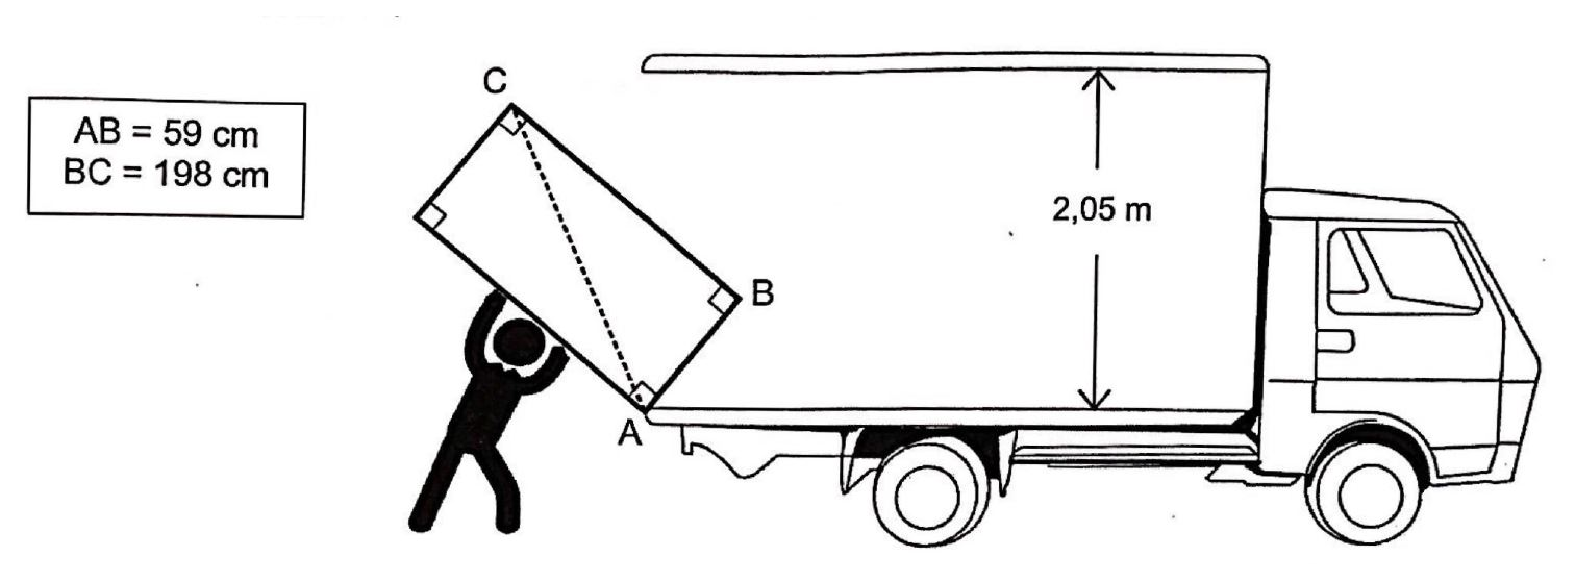
\includegraphics[width=12cm]{demenagement}
\end{center}

\smallskip

Allan pourra-t-il redresser le réfrigérateur en position verticale pour le rentrer dans le camion sans bouger le point d'appui A ? Justifier.

\subsection*{Exercice 4 \hfill \textit{15 points}}

La figure ci-dessous n'est pas réalisée en vraie grandeur. Elle n'est pas à reproduire.

\begin{center}
    \psset{unit=0.8cm}
    \begin{pspicture}(13,7)
    \psline(0,0.8)(12.8,6.6)%EACN
    \psline(0,5.8)(12.9,0.6)%MBAF
    \psline(2.9,0)(0,6.7)%NM
    \psline(4.6,0)(1.5,7)%BC
    \psline(12.5,0)(9.45,7)%EF
    \uput[dl](2.15,1.65){N} \uput[ur](0.45,5.6){M} \uput[ur](2.43,4.8){B} \uput[dl](3.55,2.3){C} 
    \uput[u](5.82,3.42){A} \uput[ur](10.1,5.5){E} \uput[dl](12.1,0.9){F} 
    \end{pspicture}
\end{center}

Les droites (BC) et (MN) sont parallèles.\\
On donne : AB = 4,5~cm ; AC = 3~cm ; AN = 4,8~cm et MN = 6,4~cm.

\begin{enumerate}
    \item[1.] Calculer AM et BC. 							
    \item[2.] On sait de plus que AE = 5~cm et AF = 7,5~cm.\\
    Montrer que les droites (EF) et (BC) sont parallèles. 			
\end{enumerate}

\subsection*{Exercice 5 \hfill \textit{11 points}}

Un chocolatier vient de fabriquer \SI{2622}{œufs} de Pâques et \SI{2530}{poissons} en chocolat.

Il souhaite vendre des paquets avec un mélange d'œufs et de poissons de façon que :

\begin{itemize}[label={$\bullet$}]
    \item Tous les paquets ont la même composition.
    \item À la fin, il ne reste ni œufs, ni poissons.
\end{itemize}

\begin{enumerate}
    \item[1.] Le chocolatier peut-il faire 19 paquets ? Justifier.
    \item[2.] Quel est le plus grand nombre de paquets qu'il peut réaliser ? \\
    Dans ce cas, quelle sera la composition de chaque paquet ?
\end{enumerate}

\newpage

\subsection*{Exercice 6 \hfill \textit{16 points}}


On demande à quinze élèves d'une classe A et à dix élèves d'une classe B de compter le nombre de SMS qu'ils envoient pendant un week-end.

Le lundi on récupère les résultats dans un tableur.

\begin{center}
    \begin{tabularx}{\linewidth}{|c|c|*{15}{>{\footnotesize \centering \arraybackslash}X|}c|c|}\hline
        &A		&B	&C	&D	&E	&F	&G	&H	&I	&J	&K	&L	&M	&N	&O	&P	&Q	&R\\ \hline
    1	&Classe&\multicolumn{15}{|c|}{Nombre de SMS envoyés par élève dans le week-end}&Moy.&Méd.\\ \hline
    2	&A		&0	&0	&0	&0	&0	&5	&7	&12	&15	&15	&16	&18	&21	&34	&67	&	&\\ \hline
    3	&B		&0	&1	&1	&2	&11	&17	&18	&18	&20	&32	&	&	&	&	&	&\footnotesize 12	&\footnotesize 14\\ \hline
    \end{tabularx}
\end{center}

\begin{enumerate}
    \item[1.] Calculer la moyenne et la médiane du nombre de SMS envoyés par ces élèves de la classe A.
    \item[2.] Quelles formules ont pu être écrites dans les cellules Q3 et R3 du tableur ?
    \item[3.] Calculer la moyenne du nombre de SMS envoyés pendant le week-end par ces 25 élèves des classes A et B.
    \item[4.] Calculer la médiane du nombre de SMS envoyés pendant le week-end par ces 25 élèves des classes A et B.
\end{enumerate}

\subsection*{Exercice 7 \hfill \textit{13 points}}

Un couple et leurs deux enfants Thomas et Anaïs préparent leur séjour au ski du 20 au 27 février.

Il réservent un studio pour 4 personnes pour la semaine.

Pendant 6 jours, Anaïs et ses parents font du ski et Thomas du snowboard. Ils doivent tous louer leur matériel.

Ils prévoient \textbf{une dépense de 500 \euro} pour la nourriture et les sorties de la semaine.

\begin{center}
	
    \begin{tabularx}{\linewidth}{|>{\centering \arraybackslash }m{3cm} | *{4}{>{\centering \arraybackslash} X |}} \cline{2-5}
        \multicolumn{1}{l |}{~}	& \textbf{06/02 - 13/02} & \textbf{13/02 - 20/02}  & \textbf{20/02 - 27/02} & \textbf{27/02 - 05/03}  \\  \hline
        Studio 4 personnes \linebreak 29~m$^2$	&  $\SI{870}{€}$ &  $\SI{1020}{€}$ & $\SI{1020}{€}$ & $\SI{1020}{€}$ \\ \hline
        T2 6  personnes \linebreak 36~m$^2$	&  $\SI{1050}{€}$ &  $\SI{1250}{€}$ & $\SI{1250}{€}$ & $\SI{1250}{€}$ \\ \hline
        T3 8 personnes \linebreak 58~m$^2$	&  $\SI{1300}{€}$ &  $\SI{1550}{€}$ & $\SI{1550}{€}$ & $\SI{1550}{€}$ \\ \hline
    \end{tabularx} 

\vspace{5mm}

    \begin{tabularx}{0.8\linewidth}{|X l|} \hline
        \multicolumn{2}{| c |}{\textbf{Location de matériel de ski :}}  \\  
        Adulte : skis, casque, chaussures : & 17~\euro~par jour \\
        Enfant : skis, casque, chaussures : & 10~\euro~par jour \\
        Enfant : snowboard, casque, chaussures : & 19~\euro~par jour \\ \hline
    \end{tabularx} 

\vspace{5mm}

    \begin{tabularx}{\linewidth}{|c | p{2mm} |X r|} \cline{1-1} \cline{3-4}
    \textbf{Formule 1}					&&\multicolumn{2}{c|}{\textbf{Formule 2}} \\
                                        && Achat d'une Carte Famille & 120~\euro \\
    1 adulte 187,50~\euro{} pour 6 jours&& \multicolumn{2}{c |}{Puis :}\\
    1 enfant 162,50~\euro{} pour 6 jours&&1 forfait adulte 				& 25~\euro~par jour \\
                                        &&1 forfait enfant 				& 20~\euro~par jour \\  \cline{1-1} \cline{3-4}
    \end{tabularx} 

\end{center}

\begin{enumerate}
	\item[1.] Déterminer pour cette famille, la formule la plus intéressante pour l'achat des forfaits pour six jours.
	\item[2.] Déterminer alors le budget total à prévoir pour leur séjour au ski.
\end{enumerate}


\end{document}